
\documentclass[conference]{IEEEtran}

% ==========================================
% Packages
% ==========================================
\usepackage{iftex}
\ifXeTeX % local preview builds (e.g., Tectonic); pdfLaTeX on Overleaf uses Times directly
  \usepackage{fontspec}
  \setmainfont{texgyretermes}[Extension=.otf, UprightFont=*-regular,
    BoldFont=*-bold, ItalicFont=*-italic, BoldItalicFont=*-bolditalic]
\fi
\usepackage{cite}
\usepackage{amsmath,amssymb,amsfonts}
\usepackage{graphicx}
\usepackage{booktabs}
\usepackage{array}
\usepackage{algorithm}
\usepackage{algpseudocode}
\usepackage{xcolor}
\usepackage{url}
\usepackage{tikz}
\usetikzlibrary{positioning,arrows.meta}

\graphicspath{{figures/}}

\begin{document}

% ==========================================
% Title
% ==========================================
\title{When to Advise and When to Defer: A Domain-Specific Tool-Grounded Agent for Departure Decisions in Curbside Waste Collection}

% ==========================================
% Authors
% ==========================================
\author{
    \IEEEauthorblockN{
        First Author and Second Author
    }
    \IEEEauthorblockA{
        Department of Computer Science and Engineering\\
        National Chung Hsing University\\
        Taichung, Taiwan\\
        Email: author@example.com
    }
}

\maketitle

% ==========================================
% Abstract and Keywords
% ==========================================
\begin{abstract}
As Taiwan enters a super-aged society, the real burden of curbside waste collection is not locating the garbage truck but deciding whether a resident, given their location and walking pace, can still leave home and arrive comfortably in time. This departure decision faces three compounding uncertainties: arrival-time prediction, walking time, and data freshness. Rather than refining arrival-time accuracy, this study defines when a system is entitled to recommend departure and when it must degrade. Using Taichung City as the study area, we build a domain-specific artificial intelligence agent that encapsulates waste-collection knowledge, including collection schedules, pedestrian network accessibility, and operational characteristics, as whitelisted tools. A large language model handles only intent recognition and explanation, whereas numerical computation and decisions are executed by controlled tools with schema-validated inputs and outputs, confining tool hallucination within verifiable boundaries. Feasibility is judged by a time margin, namely the predicted arrival time minus the walking time and a safety buffer, with the buffer adapted to data latency and prediction error; walking time is estimated with a spatial database. Rolling-origin backtesting compares historical-average, distance--speed, and regression predictors by mean absolute error and root-mean-square error, treats the false-feasibility rate as the primary safety metric, reports recommendation coverage and fallback success rate, and includes at least thirty anomaly scenarios. Expected outcomes include statistically significant improvement over the historical-average baseline, a bounded false-feasibility rate without collapse in coverage, full disclosure of data sources and fallback reasons, and an explicit applicability boundary for personalized departure advice under low-frequency data.
\end{abstract}
\begin{IEEEkeywords}
Arrival time prediction, decision support systems, domain-specific agents, graceful degradation, large language models, tool hallucination, waste collection.
\end{IEEEkeywords}


% ==========================================
% I. Introduction
% ==========================================
\section{Introduction}\label{sec:intro}

\subsection{Background and Motivation}
In many Taiwanese cities, household waste is not left at the curb but handed directly to a collection truck that stops briefly at designated points according to a published schedule. Residents must therefore be physically present at a stop within a narrow time window. Taichung City publishes the positions of its garbage and recycling trucks as open data, with records containing route, vehicle, timestamp, location, coordinates, and speed fields refreshed approximately every ten minutes~\cite{taichung_fleet_api}. Such data make it possible to see \emph{where} a truck is, but they do not answer the question residents actually face: \emph{given where I am and how fast I walk, should I leave now, and for which stop?}

This question is becoming more consequential as the population ages. Taiwan crossed the threshold of a super-aged society, in which more than 20\% of the population is aged 65 or above, in 2025~\cite{ndc_population}, and walking speed varies substantially with age~\cite{knoblauch1996}. For an older resident, leaving too early means waiting at the curb, while leaving too late means missing the truck and storing waste for another day. A departure recommendation that is wrong in the optimistic direction is therefore more harmful than no recommendation at all.

\subsection{Problem Statement and Research Gap}
A departure decision combines three uncertain quantities: the truck's arrival time at a stop, the resident's walking time to that stop, and the freshness of the data on which both estimates depend. Existing tools address these separately. Municipal applications show static schedules or the latest vehicle icon but do not intersect vehicle arrival with pedestrian walking time. General navigation services estimate walking routes but have no model of collection-route logic or dwell behavior at stops. Large language models (LLMs) can converse naturally about the problem, but without grounded access to live data and spatial computation they may produce plausible yet fabricated times and distances~\cite{ji2023hallucination}.

Prior work on vehicle arrival prediction largely treats the task as improving point accuracy~\cite{chien2002,jeong2004}. With location updates arriving only every ten minutes, however, accuracy has a hard ceiling, and the more useful question becomes one of \emph{abstention}: under what data conditions is a system entitled to tell a user to leave, and when must it decline and fall back to less specific information? This framing follows the classical reject option in decision theory~\cite{chow1970} and selective prediction~\cite{geifman2017}, but to our knowledge it has not been applied to curbside collection or to tool-using LLM agents for municipal services.

\subsection{Research Contributions}
This paper presents \emph{GarbageGo}, a domain-specific, tool-grounded agent for departure decisions in curbside waste collection in Taichung City. Its contributions are as follows:
\begin{itemize}
\item \textbf{An advise-or-defer decision formulation.} We define departure feasibility through a time margin (slack) between predicted truck arrival, estimated walking time, and a safety buffer that widens with data latency, prediction error, and positioning uncertainty, together with explicit conditions under which the system must defer rather than advise.
\item \textbf{A tool-grounded agent architecture.} Domain knowledge, including schedules, pedestrian accessibility, and collection-operation characteristics, is encapsulated as whitelisted tools with JSON Schema-validated inputs and outputs. The LLM is restricted to intent recognition and explanation, and every number it reports must originate from a tool result.
\item \textbf{A safety-oriented evaluation protocol.} We specify a rolling-origin backtest that compares arrival-time predictors, treats the false-feasibility rate as the primary safety metric alongside recommendation coverage and fallback success, and includes at least thirty anomaly scenarios covering stale data, API failure, positioning error, and out-of-scope requests.
\end{itemize}
This paper reports the problem formulation, system design, and evaluation protocol. Empirical results will be reported after the backtest is completed; no experimental values are claimed here.

\subsection{Paper Organization}
Section~\ref{sec:related} reviews related work. Section~\ref{sec:method} presents the proposed scheme. Section~\ref{sec:experiments} describes the evaluation design, and Section~\ref{sec:conclusion} concludes the paper.


% ==========================================
% II. Related Work
% ==========================================
\section{Related Work}\label{sec:related}

Following the dual nature of the problem, this section reviews existing methods from simple to complex, covering both domain knowledge on collection operations and AI techniques for agents and selective decisions, and then summarizes them in a SWOT comparison.

% M. Methods
\subsection{Existing Methods}
\textbf{Collection schedules and operations.} Operations research on municipal solid waste collection has focused on the operator's side: vehicle routing, districting, and scheduling~\cite{belien2014}. Published schedules are its resident-facing product. They are easy to understand, but actual arrivals drift with traffic, weather, and variable dwell times along the route. Open fleet feeds such as Taichung's~\cite{taichung_fleet_api} add live positions but leave the interpretation to residents.

\textbf{Arrival-time prediction.} For fixed-route vehicles, arrival times have been predicted with historical averages, regression, Kalman filtering, and neural networks~\cite{chien2002,jeong2004}. These methods generally assume dense location updates and evaluate point accuracy. With sparse observations, simple baselines may be as robust as complex models, and a fair comparison requires time-ordered evaluation that prevents information from the future leaking into training~\cite{tashman2000,hyndman2021}.

\textbf{Pedestrian accessibility.} Walking time depends on the pedestrian network rather than straight-line distance, and walking speed differs substantially across individuals and age groups~\cite{knoblauch1996}. Spatial databases such as PostGIS support indexed nearest-neighbor search and network distance computation for many candidate stops per query~\cite{postgis}.

\textbf{Tool-using LLM agents.} LLMs can be extended with external tools by interleaving reasoning and actions~\cite{yao2023react}, by learning when to call application programming interfaces~\cite{schick2023toolformer}, or by fine-tuning on large API collections~\cite{patil2023gorilla}. Tool use reduces but does not eliminate hallucination: models may still invent arguments, misreport tool outputs, or answer outside their competence~\cite{ji2023hallucination}.

% N. New proposed
\subsection{New Trends and the Proposed Direction}
Two recent trends motivate this work. First, deployed agents are moving from open-ended tool use toward restricted, schema-validated tool sets, trading flexibility for verifiability. Second, selective prediction formalizes when a model should abstain through a risk--coverage trade-off~\cite{chow1970,geifman2017}. GarbageGo combines both: it restricts the LLM to explaining the output of validated domain tools, and it treats departure advice as a selective decision whose primary measure is the false-feasibility rate at a given coverage rather than arrival-time accuracy alone.

% O. Organize
\subsection{Comparative Summary}
Table~\ref{tab:swot} summarizes the strengths, weaknesses, opportunities, and threats of the four method families with respect to departure decisions.

\begin{table*}[t]
\caption{SWOT Comparison of Existing Approaches for Departure Decisions in Curbside Collection}
\label{tab:swot}
\centering
\footnotesize
\begin{tabular}{@{}p{0.15\textwidth}p{0.19\textwidth}p{0.19\textwidth}p{0.19\textwidth}p{0.19\textwidth}@{}}
\toprule
Approach & Strengths & Weaknesses & Opportunities & Threats \\
\midrule
Static schedules and tracking displays~\cite{belien2014,taichung_fleet_api} & Simple, transparent, available citywide & No walking time; no estimate of arrival at the user's stop & Open fleet feeds enable dynamic services & Drift from schedule misleads residents \\
\addlinespace
Arrival-time prediction~\cite{chien2002,jeong2004} & Quantitative ETA with measurable error & Assumes dense data; gives an estimate, not a departure decision & Historical feeds allow backtesting & Ten-minute updates cap accuracy; overfitting \\
\addlinespace
Pedestrian routing~\cite{knoblauch1996,postgis} & Network-based walking time, per-user speed & Ignores truck route and dwell behavior & Spatial databases scale to many stops & Positioning error; age-related speed variation \\
\addlinespace
Tool-using LLM agents~\cite{yao2023react,schick2023toolformer,patil2023gorilla} & Natural-language interaction and flexible orchestration & Hallucinated numbers; unbounded tool use~\cite{ji2023hallucination} & Schema-validated tools and grounding checks & Unsafe advice; out-of-scope answers \\
\bottomrule
\end{tabular}
\end{table*}


% ==========================================
% III. Proposed Scheme
% ==========================================
\section{Proposed Scheme}\label{sec:method}

% PA. Aim
\subsection{Design Aim}
GarbageGo aims to answer one question for a resident at query time $t_q$: \emph{which nearby stop, if any, can I safely reach before the truck if I leave now?} The design goals are (G1) to rank stops by the safety of reaching them rather than by distance; (G2) to keep the rate of wrong ``you can make it'' advice below a target level; (G3) to defer explicitly when data do not support advice; and (G4) to ensure that every number shown to the user comes from a verifiable computation.

% PB. Based on / background
\subsection{Background and Design Basis}
The design rests on four domain facts. First, the Taichung fleet feed is refreshed about every ten minutes, and each record has an observation time $t_o$ (\texttt{observed\_at}) and a time $t_c$ (\texttt{collected\_at}) at which GarbageGo receives it~\cite{taichung_fleet_api}. Second, trucks follow fixed routes with short dwell times at each stop, so a truck that has passed a stop will not return. Third, the nearest stop is often the one the truck is about to leave. Fourth, walking speed varies widely, especially among older adults~\cite{knoblauch1996}.

% PC. Cure / Cause
\subsection{Rationale of the Solution}
Because sparse data place a ceiling on arrival-time accuracy, GarbageGo does not try to make the estimate exact. Instead, it carries the uncertainty explicitly into the decision: a safety buffer absorbs latency, prediction error, and positioning error, and the system abstains when the uncertainty is too large. This works because a miss can only occur when the combined estimation error exceeds the buffer, which is shown formally in Section~\ref{subsec:math}.

% PD. Design paradigm
\subsection{Design Paradigm}
The design combines two shifts. The first is from \emph{prediction} to \emph{selective decision}: the output is not an arrival time but one of three outcomes, namely advise, no feasible stop, or defer. The second is from \emph{open-ended} to \emph{tool-grounded} agents: the LLM interprets requests and explains results, while all spatial and temporal computation is done by deterministic, schema-validated tools.

% PE. Paper elements
\subsection{System Elements}
GarbageGo is implemented as a modular monolith, a single deployable service with strict internal module boundaries, backed by PostgreSQL with the PostGIS extension~\cite{postgis} and exposed through a FastAPI web interface. Its elements are: (E1) a \emph{data acquisition and validation} module that ingests live and historical fleet records with the same format, checks fields, coordinate ranges, and timestamps, and stores both $t_o$ and $t_c$; (E2) a \emph{GIS engine} that retrieves candidate stops and computes network walking distances; (E3) an \emph{ETA engine} with interchangeable predictors; (E4) a \emph{recommendation engine} that applies the decision rule; and (E5) an \emph{LLM agent} that may call only the whitelisted tools in Table~\ref{tab:tools}.

\begin{table}[t]
\caption{Whitelisted Tools Exposed to the LLM Agent}
\label{tab:tools}
\centering
\footnotesize
\begin{tabular}{@{}lp{0.47\columnwidth}@{}}
\toprule
Tool & Output \\
\midrule
\texttt{find\_candidate\_stops} & Stops within radius whose collection window covers $t_q$ \\
\texttt{get\_fleet\_status} & Latest truck records with $t_o$, $t_c$, and validation flags \\
\texttt{estimate\_walking\_time} & $\hat{W}_s$ from network distance and $v_u$ \\
\texttt{predict\_eta} & $\hat{A}_s$ and residual spread $\hat{e}_s(h)$ \\
\texttt{evaluate\_feasibility} & Outcome (advise, defer, or no feasible stop), ranked stops, $\sigma_s$, reasons \\
\texttt{get\_static\_timetable} & Published schedule for the fallback mode \\
\bottomrule
\end{tabular}
\end{table}

% PF. Formulation
\subsection{Formulation}
A resident at location $u$ with walking speed $v_u$ issues a query at $t_q$. Let $\mathcal{S}$ be the set of stops within a search radius of $u$ whose collection window covers $t_q$. The data latency is
\begin{equation}
\Delta = t_q - t_o ,
\label{eq:latency}
\end{equation}
which includes both the update interval and the transmission delay $t_c - t_o$. For each stop $s\in\mathcal{S}$, the ETA engine estimates the remaining time $\hat{A}_s$ until the truck arrives, and the GIS engine estimates the walking time
\begin{equation}
\hat{W}_s = \frac{d_{\mathrm{net}}(u,s)}{v_u},
\label{eq:walk}
\end{equation}
where $d_{\mathrm{net}}$ is the shortest pedestrian-network distance. The \emph{slack} of stop $s$ is
\begin{equation}
\sigma_s = \hat{A}_s - \hat{W}_s - B_s ,
\label{eq:slack}
\end{equation}
with the safety buffer
\begin{equation}
B_s = b_0 + \alpha\,\Delta + z\,\hat{e}_{s}(h) + \frac{\epsilon_u}{v_u},
\label{eq:buffer}
\end{equation}
where $b_0$ is a minimum buffer (initially three minutes); $\alpha\Delta$ accounts for truck movement since the last observation; $\hat{e}_{s}(h)$ is the empirical spread of arrival-time residuals at prediction horizon $h$, estimated on training data; $z$ sets the conservativeness; and $\epsilon_u$ is the positioning accuracy reported by the user's device. A positive slack means that, under current data, the resident can leave now and arrive with at least $B_s$ to spare, and $t_q + \sigma_s$ is the latest recommended departure time.

The decision rule returns exactly one outcome. \textbf{Defer:} if fleet data are unavailable, invalid, or stale ($\Delta > \tau$, with $\tau = 15$ minutes initially), slack is not computed; the official static schedule is shown with an explicit statement of why dynamic advice is unavailable. \textbf{Advise:} otherwise, stops already passed by the truck are removed, and if the feasible set $\mathcal{F} = \{s : \sigma_s > 0\}$ is non-empty, stops are ranked by slack in descending order, giving one primary recommendation and up to two alternatives. \textbf{No feasible stop:} if $\mathcal{F}$ is empty, the system says so and shows the next scheduled collection.

The ETA engine exposes four predictors behind a common interface: (i) the \emph{static schedule}; (ii) the \emph{historical average} travel time from the truck's current route position to $s$ for the same route, weekday type, and time of day; (iii) a \emph{distance--speed} model using remaining route distance, recent speed, and expected dwell at intermediate stops; and (iv) a \emph{regression} model over remaining route distance, number of remaining stops, time of day, weekday type, recent speed, and latency. All predictors project the truck position onto the ordered stop sequence of its route; a truck reporting zero speed for an extended period is flagged as stationary, and its uncertainty term is widened.

% PG. Graph
\subsection{Architecture}
Fig.~\ref{fig:architecture} shows how the elements interact. The only probabilistic component, the LLM agent, sits between the user and the deterministic engines. It sends schema-validated tool calls and receives a structured JSON result. The GIS and ETA engines supply $\hat{W}_s$ and $\hat{A}_s$ to the recommendation engine, and the validation module supplies the latency $\Delta$ that drives both the buffer and the defer decision.

\begin{figure}[t]
\centering
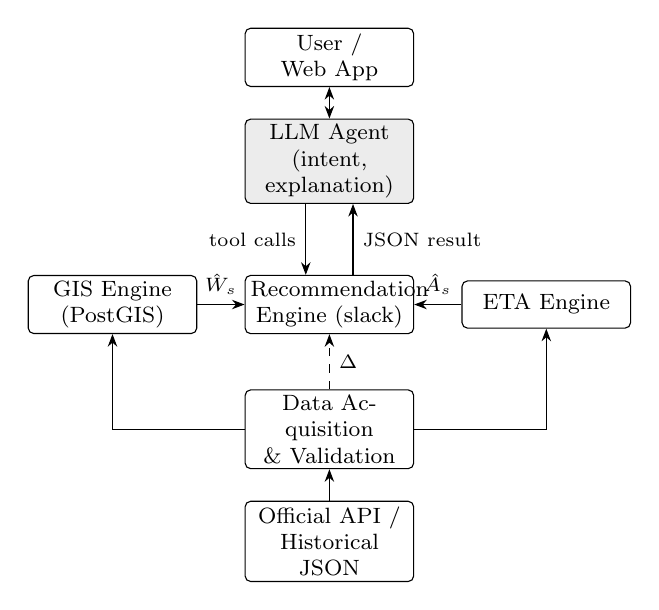
\begin{tikzpicture}[
  node distance=4mm and 6mm,
  box/.style={draw, rounded corners=2pt, align=center, font=\footnotesize,
              minimum height=6mm, inner sep=2pt, text width=20mm},
  llm/.style={box, fill=gray!15},
  arr/.style={-{Stealth[length=1.6mm]}, thin}]
\node[box] (user) {User / Web App};
\node[llm, below=of user] (agent) {LLM Agent\\(intent, explanation)};
\node[box, below=9mm of agent] (rec) {Recommendation\\Engine (slack)};
\node[box, left=of rec] (gis) {GIS Engine\\(PostGIS)};
\node[box, right=of rec] (eta) {ETA Engine};
\node[box, below=7mm of rec] (val) {Data Acquisition\\\& Validation};
\node[box, below=of val] (src) {Official API /\\Historical JSON};
\draw[{Stealth[length=1.6mm]}-{Stealth[length=1.6mm]}, thin] (user) -- (agent);
\draw[arr] ([xshift=-3mm]agent.south) -- node[left, font=\scriptsize]{tool calls} ([xshift=-3mm]rec.north);
\draw[arr] ([xshift=3mm]rec.north) -- node[right, font=\scriptsize]{JSON result} ([xshift=3mm]agent.south);
\draw[arr] (gis) -- node[above, font=\scriptsize]{$\hat{W}_s$} (rec);
\draw[arr] (eta) -- node[above, font=\scriptsize]{$\hat{A}_s$} (rec);
\draw[arr] (src) -- (val);
\draw[arr] (val.west) -| (gis.south);
\draw[arr] (val.east) -| (eta.south);
\draw[arr, dashed] (val) -- node[right, font=\scriptsize]{$\Delta$} (rec);
\end{tikzpicture}
\caption{GarbageGo architecture. Shaded: probabilistic language component; unshaded: deterministic, schema-validated tools. All numbers shown to the user originate from deterministic tools.}
\label{fig:architecture}
\end{figure}

% PH. How
\subsection{How the Design Goals Are Achieved}
Goal G1 is met by ranking on $\sigma_s$ instead of distance and by excluding stops already passed. G2 is met by the buffer~\eqref{eq:buffer}, whose parameters $\alpha$ and $z$ are calibrated on the training period so that the false-feasibility rate on validation data stays below a target $\eta$, as justified in Section~\ref{subsec:math}. G3 is met by the defer outcome, triggered by staleness, validation failure, or unavailable data, always with a disclosed reason. G4 is met by tool grounding: each tool has a JSON Schema for its arguments and result, invalid calls are rejected before execution, the response is generated from the result payload under a grounding template, and every number in the generated text is checked against that payload. If the check fails, a deterministic text template is used instead. Out-of-domain requests, such as medical questions, are declined by rule.

% PI. Implementation / interaction
\subsection{Implementation and Interaction}
Algorithm~\ref{alg:method} gives the end-to-end procedure executed for each query.

\begin{algorithm}[t]
\caption{Advise-or-Defer Departure Recommendation}
\label{alg:method}
\begin{algorithmic}[1]
\Require user location $u$, walking speed $v_u$, query time $t_q$
\Ensure outcome, ranked stops with slack, explanation
\State $\mathcal{S} \gets$ \Call{FindCandidateStops}{$u, t_q$}
\State $D \gets$ \Call{GetFleetStatus}{$\mathcal{S}$}
\If{$D$ is unavailable or invalid \textbf{or} $t_q - t_o > \tau$}
  \State \Return \Call{Explain}{\textsc{Defer}, \Call{StaticTimetable}{$\mathcal{S}$}, reason}
\EndIf
\State $\mathcal{F} \gets \emptyset$
\ForAll{$s \in \mathcal{S}$ not yet passed by the truck}
  \State $\hat{W}_s \gets$ \Call{WalkingTime}{$u, s, v_u$}
  \State $(\hat{A}_s, \hat{e}_s) \gets$ \Call{PredictETA}{$s, D$}
  \State $B_s \gets b_0 + \alpha\Delta + z\,\hat{e}_s + \epsilon_u / v_u$
  \State $\sigma_s \gets \hat{A}_s - \hat{W}_s - B_s$
  \If{$\sigma_s > 0$} \State $\mathcal{F} \gets \mathcal{F} \cup \{(s,\sigma_s)\}$ \EndIf
\EndFor
\If{$\mathcal{F} = \emptyset$}
  \State \Return \Call{Explain}{\textsc{NoFeasibleStop}, next schedule}
\EndIf
\State sort $\mathcal{F}$ by $\sigma_s$ in descending order
\State \Return \Call{Explain}{\textsc{Advise}, top three of $\mathcal{F}$, $\Delta$}
\end{algorithmic}
\end{algorithm}

% PJ. Jump to an example
\subsection{Illustrative Example}
Table~\ref{tab:example} walks through a hypothetical query; the values are chosen for illustration and are not measurements. A resident walking at 1.0~m/s queries three stops with fleet data that are six minutes old ($\Delta = 6$~min $\le \tau$), a device accuracy of 30~m (0.5~min of walking), $b_0 = 3$~min, $\alpha = 0.2$, and error terms $z\hat{e}_s$ of 1.0, 1.8, and 2.4~min for stops A, B, and C, whose prediction horizons grow in that order. Stop~A is the nearest, and the resident could physically walk there before the truck's predicted arrival ($2.5 < 4$~min). However, once the buffer is included its slack is negative, so it is rejected. Stop~B has the largest slack and becomes the primary recommendation, with a latest departure time 2.5~min after the query, and stop~C is offered as an alternative. If the same query arrived with $\Delta = 18$~min, the system would defer and show the static schedule instead.

\begin{table}[t]
\caption{Illustrative Example with Hypothetical Values (Minutes)}
\label{tab:example}
\centering
\footnotesize
\begin{tabular}{@{}lcccccl@{}}
\toprule
Stop & $d_{\mathrm{net}}$ (m) & $\hat{A}_s$ & $\hat{W}_s$ & $B_s$ & $\sigma_s$ & Decision \\
\midrule
A & 150 & 4.0 & 2.5 & 5.7 & $-4.2$ & Rejected \\
B & 420 & 16.0 & 7.0 & 6.5 & 2.5 & Primary \\
C & 600 & 19.0 & 10.0 & 7.1 & 1.9 & Alternative \\
\bottomrule
\end{tabular}
\end{table}

% PK. Key points
\subsection{Key Points}
The scheme contributes (i) a slack-based, selective decision that ranks stops by safety margin and can abstain; (ii) a buffer that grows with each identified source of uncertainty, with a calibration target tied to the false-feasibility rate; and (iii) a tool-grounded agent in which language generation cannot introduce unverified numbers.

% PL. Later how to do simulation
\subsection{Simulation Plan}
The scheme is evaluated by replaying 2024--2026 historical fleet records in time order. Simulated residents with different walking speeds query from origins around each stop, and outcomes are compared with reference arrivals reconstructed from the records. Section~\ref{sec:experiments} gives the full protocol.

% PM. Math proof
\subsection{Analysis of the False-Feasibility Rate}\label{subsec:math}
Let $A_s$ and $W_s$ be the true remaining arrival time and walking time, and let $x$ denote all information available at $t_q$, which determines $\hat{A}_s$, $\hat{W}_s$, $B_s$, and hence whether stop $s$ is advised. Ignoring dwell time (which only helps the resident), a resident who leaves at $t_q$ misses the truck if $A_s < W_s$. Define the combined error
\begin{equation}
E_s = (\hat{A}_s - A_s) + (W_s - \hat{W}_s).
\label{eq:error}
\end{equation}

\textbf{Proposition 1.} If $B_s \ge q_{1-\eta}(E_s \mid x)$, the $(1-\eta)$ conditional quantile of $E_s$, then $\Pr(\text{miss} \mid \text{advise}) \le \eta$.

\emph{Proof.} Stop $s$ is advised only if $\hat{A}_s - \hat{W}_s > B_s$. A miss means $A_s - W_s < 0$. Subtracting the second inequality from the first gives $E_s > B_s$, so for every $x$ in which $s$ is advised, $\Pr(\text{miss} \mid x) \le \Pr(E_s > B_s \mid x) \le \eta$. Since advising is determined by $x$, averaging over all such $x$ gives $\Pr(\text{miss} \mid \text{advise}) \le \eta$. \hfill$\blacksquare$

\textbf{Proposition 2.} For fixed estimates $\hat{A}_s$ and $\hat{W}_s$, increasing the buffer of every stop cannot enlarge the feasible set $\mathcal{F}$, so coverage is non-increasing in $z$, $\alpha$, and $b_0$.

\emph{Proof.} $\sigma_s$ is strictly decreasing in $B_s$, and $B_s$ is non-decreasing in each of these parameters. Hence any stop with $\sigma_s \le 0$ under a smaller buffer still has $\sigma_s \le 0$ under a larger one. \hfill$\blacksquare$

Together, the propositions show that the buffer is a single control for the risk--coverage trade-off~\cite{geifman2017}. The terms of~\eqref{eq:buffer} serve as a practical estimate of $q_{1-\eta}(E_s \mid x)$. Because this quantile is estimated, the bound holds only approximately, which is why the false-feasibility rate is measured directly in the backtest.


% ==========================================
% IV. Experiments and Discussion
% ==========================================
\section{Evaluation Design}\label{sec:experiments}

This section specifies the evaluation protocol. The backtest has not yet been executed, so no measured values are reported; Table~\ref{tab:comparison} shows the planned reporting format.

\subsection{Data and Ground Truth}
The evaluation uses historical Taichung fleet records collected from the open-data feed~\cite{taichung_fleet_api} over 2024--2026, which share the format of the live API, together with published collection schedules and stop locations. Before use, records are validated for missing fields, coordinates outside the city boundary, duplicate timestamps, and implausible speeds, and each record keeps both $t_o$ and $t_c$.

Because positions are sampled roughly every ten minutes, the true arrival time at a stop is itself not observed directly. We define the reference arrival time as the time at which the truck's route progress, linearly interpolated between consecutive records, reaches the stop. Arrivals whose bracketing records are too far apart are excluded and reported separately. The resulting label resolution limits the accuracy that any predictor can demonstrate and is reported alongside the results.

\subsection{Rolling-Origin Backtest}
Random cross-validation would leak future traffic conditions into training. We therefore use rolling-origin evaluation~\cite{tashman2000,hyndman2021}. Records from January 2024 to December 2025 are used for model fitting and for calibrating the buffer parameters $\alpha$ and $z$, and 2026 records are held out for testing. In the test period, the system is replayed forward in time: at each simulated query time, only records with $t_c \le t_q$ are visible, and the replayed latency reproduces the actual update gaps of the feed. Simulated queries are generated from origins sampled around each stop, at several walking speeds that represent different age groups~\cite{knoblauch1996}.

\subsection{Baselines}
Arrival-time predictors are compared under identical inputs: (B1) the static schedule, (B2) the historical average, (B3) the distance--speed model, and (P) the regression model described in Section~\ref{sec:method}. For the decision layer, slack-based ranking with the adaptive buffer is compared with nearest-stop ranking and with a fixed buffer of $b_0$.

\subsection{Evaluation Metrics}
\textbf{Prediction accuracy.} Mean absolute error (MAE) and root-mean-square error (RMSE) of $\hat{A}_s$, stratified by prediction horizon and by data latency. Improvement over the historical-average baseline is tested with the Diebold--Mariano test~\cite{diebold1995}.

\textbf{Decision safety.} The primary metric is the \emph{false-feasibility rate} (FFR), the fraction of \textsc{Advise} outcomes for which the reference arrival occurs before the resident would have reached the stop:
\begin{equation}
\mathrm{FFR} = \frac{\left|\{\text{advised and missed}\}\right|}{\left|\{\text{advised}\}\right|}.
\label{eq:ffr}
\end{equation}

\textbf{Usefulness.} \emph{Coverage} is the fraction of queries receiving an \textsc{Advise} outcome, and the \emph{catch rate} is the fraction of advised queries in which the resident arrives in time. Following the risk--coverage view of selective prediction~\cite{geifman2017}, we report FFR as a function of coverage by varying $z$, so that a low FFR cannot be obtained simply by advising almost never.

\textbf{Degradation.} The \emph{fallback success rate} is the fraction of anomalous inputs for which the system correctly returns \textsc{Defer} with an accurate reason, rather than advising on invalid data.

\begin{table}[t]
\caption{Planned Comparison of Arrival-Time Predictors (Results Pending)}
\label{tab:comparison}
\centering
\begin{tabular}{lcccc}
\toprule
Predictor & MAE & RMSE & FFR & Coverage \\
\midrule
B1: Static schedule & -- & -- & -- & -- \\
B2: Historical average & -- & -- & -- & -- \\
B3: Distance--speed & -- & -- & -- & -- \\
P: Regression & -- & -- & -- & -- \\
\bottomrule
\end{tabular}
\end{table}


\subsection{Anomaly Scenario Tests}
Beyond the backtest, at least thirty anomaly scenarios test the agent end to end. They are grouped into the categories in Table~\ref{tab:anomaly}. Each scenario specifies the input, the expected outcome, and the expected disclosed reason, and is judged as passing only if no number in the response lacks a source in the tool payload.

\begin{table}[t]
\caption{Anomaly Scenario Categories}
\label{tab:anomaly}
\centering
\footnotesize
\begin{tabular}{@{}p{0.27\columnwidth}p{0.66\columnwidth}@{}}
\toprule
Category & Example and expected behavior \\
\midrule
Stale or missing data & Feed older than $\tau$ or API timeout $\rightarrow$ \textsc{Defer} with static schedule \\
Invalid records & Coordinates outside city, missing fields $\rightarrow$ record rejected \\
Stationary truck & Zero speed for an extended period $\rightarrow$ widened buffer and risk note \\
Truck already passed & Stop behind truck on route $\rightarrow$ stop excluded \\
Poor user positioning & Accuracy radius of 200~m $\rightarrow$ larger buffer, prompt to confirm location \\
Outside collection window & No active stop $\rightarrow$ next scheduled collection \\
Ambiguous or adversarial query & Missing location, prompt injection $\rightarrow$ clarification or refusal \\
Out-of-scope request & Medical question $\rightarrow$ declined by rule \\
\bottomrule
\end{tabular}
\end{table}

\subsection{Threats to Validity}
The ten-minute sampling interval bounds both prediction accuracy and label precision. Walking speeds are simulated rather than measured from users, and stop--route mapping may be incomplete for some routes. These limitations are reported explicitly rather than hidden by aggregate metrics.


% ==========================================
% V. Conclusion
% ==========================================
\section{Conclusion}\label{sec:conclusion}
This paper reframed curbside waste-collection assistance from predicting where the garbage truck is to deciding whether a resident should leave now, and when a system should decline to say. GarbageGo combines a slack-based feasibility rule with an adaptive safety buffer, an explicit defer path for stale or invalid data, and a tool-grounded agent in which the language model only interprets requests and explains results computed by validated tools. We also specified a rolling-origin evaluation that treats the false-feasibility rate as the primary safety metric, reports it against coverage, and adds at least thirty anomaly scenarios.

The expected outcomes are a statistically significant improvement in arrival-time error over the historical-average baseline, a bounded false-feasibility rate without collapse in coverage, and full disclosure of data sources and fallback reasons. These outcomes remain to be verified. Future work will complete the backtest on 2024--2026 Taichung data, measure walking speeds with real users including older adults, and use the results to delimit explicitly when personalized departure advice is justified under low-frequency fleet data.


% ==========================================
% Acknowledgment (Optional)
% ==========================================
% \section*{Acknowledgment}

% ==========================================
% References
% ==========================================
\bibliographystyle{IEEEtran}
\bibliography{references}

\end{document}